\documentclass[tikz,border=1pt,convert=pdf2svg]{standalone}
\usepackage{laser_cut}

\newcommand\motorradius{1.46in/2}
\newcommand\spacing{\ledradius+0.5mm}
\newcommand\drawpair[2]{
	\draw (#1:#2)++(#1+90:\spacing) circle (\ledradius);
	\draw (#1:#2)++(#1-90:\spacing) circle (\ledradius);
}
\newcommand\angleoffset{15}

% lab motor
\renewcommand\motorradius{1.22in}
\renewcommand\angleoffset{90}

\begin{document}
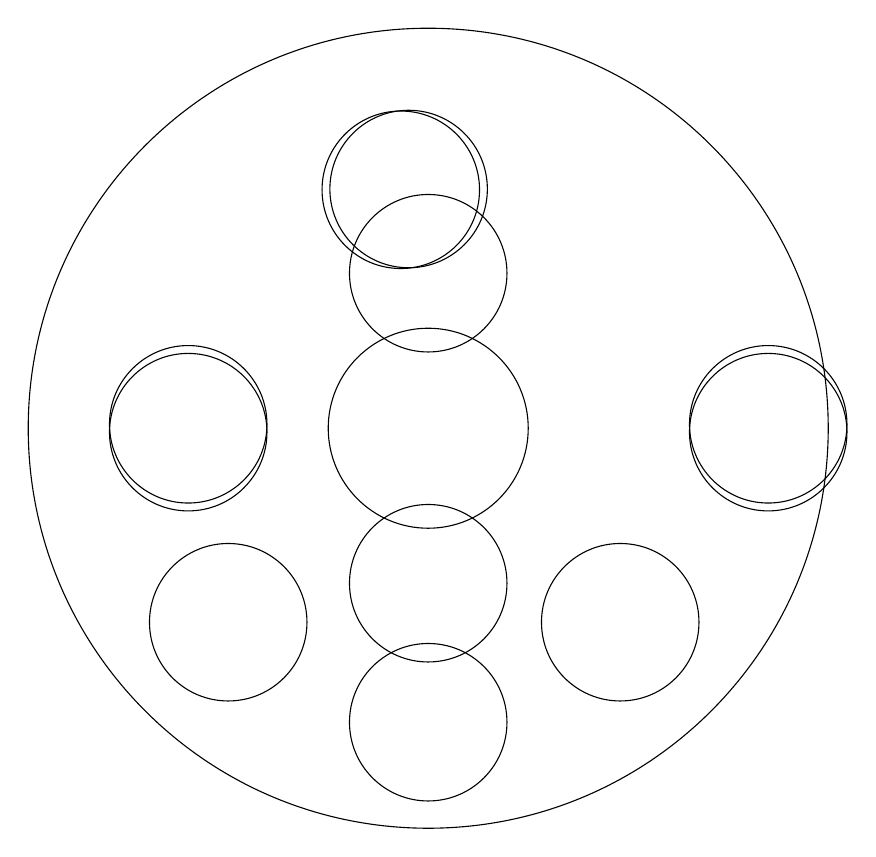
\begin{tikzpicture}
	\node (origin) at (0,0) {};
	\draw (origin) circle (4in/2); % size
	\draw (0.96in,-\motorradius+0.25in) circle (\sixthirtytworadius); % right frame hole
	\draw (-1in,-\motorradius+0.25in) circle (\sixthirtytworadius); % left frame hole
	\draw (0,-\motorradius-0.25in) circle (\sixthirtytworadius); % bottom frame hole

	% amazon motor
	% \draw (origin) circle (12mm/2); % center
	% \foreach \theta in {30,90,...,330} {
		% \draw (origin)++(\theta:31mm/2) circle (\mthreefiveradius);
	% }

	% lab motor
	\draw (origin) circle (1in/2); % center
	\foreach \theta in {-90,90} {
		\draw (origin)++(\theta:1.55in/2) circle (\eightthirtytworadius);
	}

	\drawpair{\angleoffset+90}{1.2in}
	\drawpair{\angleoffset+360/64}{1.2in}
	\drawpair{\angleoffset-90}{1.7in}
\end{tikzpicture}
\end{document}

